\section{Software Architecture of a \salespoint{} Application}
Software often need to be adaptive, flexible, and extendable.
Using a suitable architecture pattern, such as the Model-View-Controller pattern, helps to meet these non-functional requirements.
Figure \ref{sp5-arch} gives an overview of how a \salespoint{} application is modelled.
\salespoint{}, as domain framework, takes the place of the model in the MVC pattern.
The model can be extended by sub-classing \salespoint{} classes or by introducing entirely new classes.
\salespoint{} model classes and sub-classes thereof are transparently stored in a database.
If new classes are added to the model and their state is also required to be persistent, the developer also has to facilitate persisting those objects using the JPA-API.

\begin{figure}[ht]
	\centering
  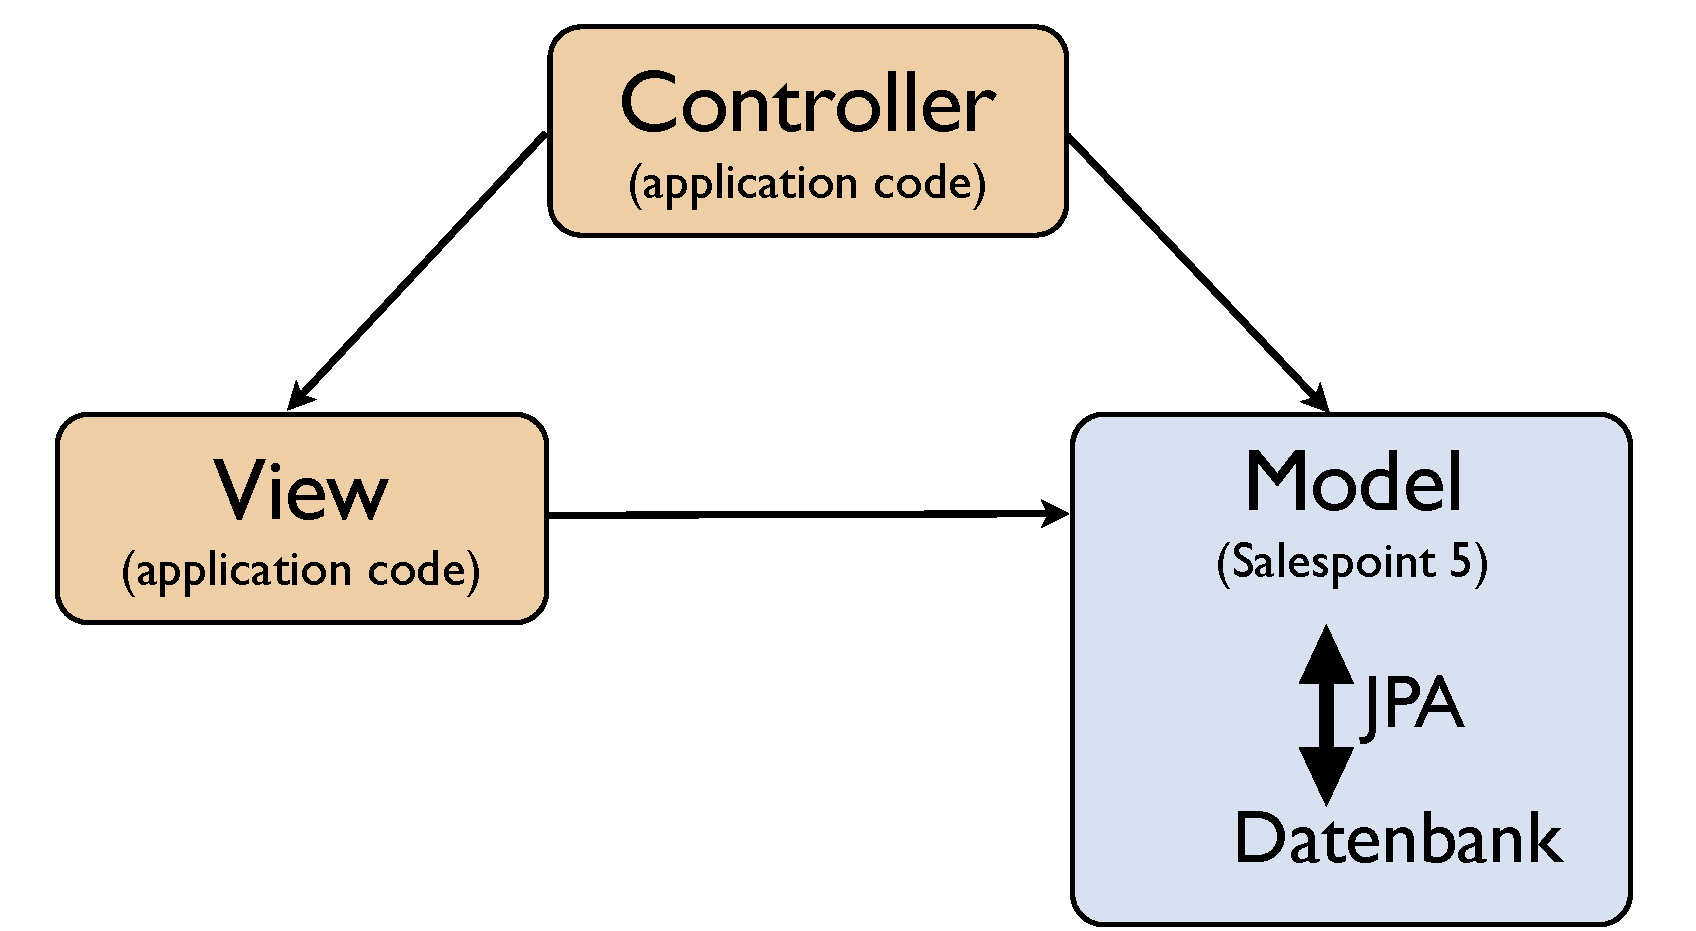
\includegraphics[width=0.6\textwidth]{images/sp5-arch.pdf}
	\label{sp5-arch}
	\caption[Overview of a \salespoint{} application.]{MVC-pattern of a \salespoint{} application divided into application specific code (red) and framework code (blue).}
\end{figure}

The controller and view are application-specific and have to be implemented by the user.
Although \salespoint{} does not require a specific framework or API like Swing~\cite{swing} or SWT~\cite{swt}.
However, because \salespoint{} is intended to be used in conjunction with the Spring MVC~\cite{spring} framework for SWP at TU Dresden, \salespoint{} contains supplementary code, easing the development of Spring applications.
This supplementary code consists of Spring MVC \code{PropertyEditor}s, and custom, \salespoint{} specific JSP-tags.
\\

\begin{figure}[ht]
	\centering
  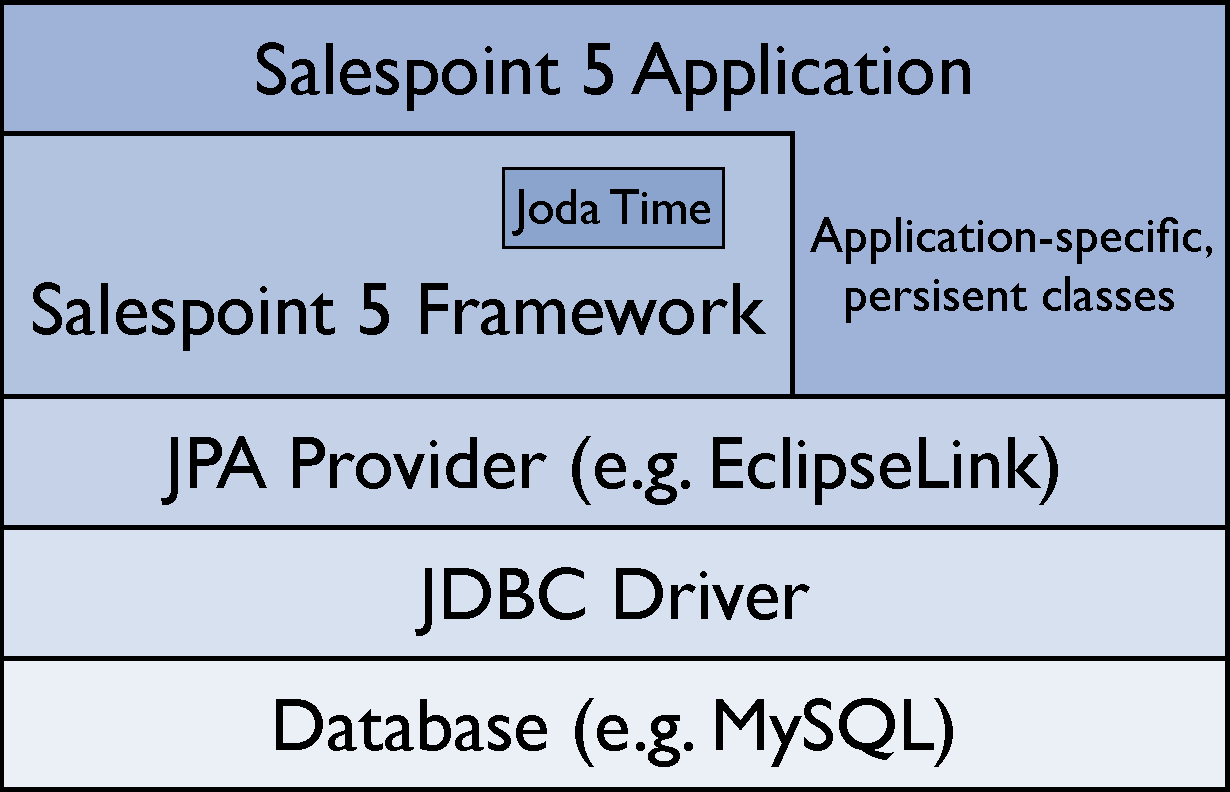
\includegraphics[width=0.45\textwidth]{images/sp5-layered.pdf}
	\label{sp5-layered}
	\caption{Layers of a \salespoint{} application.}
\end{figure}
A layered view of the software architecture of a \salespoint{} application is shown in Figure \ref{sp5-layered}.
The bottom layer corresponds to a DBMS, chosen by the developer.
As stated in Section \ref{sec:jpa}, JPA works with every DBMS for which a JDBC driver is available.
The JPA provider, which is also chosen by the developer, interfaces with the JDBC driver and \salespoint{}.
\salespoint{} in turn uses a class library, namely Joda Time~\cite{jodatime}, to deal with dates and times.
